\documentclass[12 pt,a4paper,twocolumn]{article}
\usepackage[utf8]{inputenc}
\usepackage[T1]{fontenc}
\usepackage[italian,english]{babel}
\usepackage{indentfirst} 
\usepackage{graphicx}
\usepackage{tabularx}
\usepackage{siunitx}
\usepackage{amsmath,stix,bm}
\usepackage{eucal}
\usepackage{caption}

\usepackage{multicol}
\usepackage[includeheadfoot,margin=0.7in,top=0.3 in,bottom=0.35in]{geometry}
%Per grafica vettoriale tramite InkScape%
\usepackage{color}
\usepackage{transparent}
\graphicspath{{img/}}
\usepackage[dvipsnames]{xcolor}
\usepackage{pdfpages}
\usepackage{pgfplots}
\usepackage{textcomp}

\usepackage{xcolor,colortbl}
\usepackage{listings}
\usepackage{cleveref}
\usepackage{caption}
\DeclareCaptionFont{quack}{}
\captionsetup[figure]{font={color=gray,small},labelfont={color=black,sc}}
\captionsetup[table]{font={color=gray,small},labelfont={color=black,sc}}
\captionsetup[subfigure]{font={color=gray,small},labelfont={color=black}}
\addto\captionsenglish{\renewcommand{\figurename}{Fig.}}
\addto\captionsenglish{\renewcommand{\tablename}{Tab.}}
\addto\captionsitalian{\renewcommand{\tablename}{Tab.}}
\crefname{table}{Tab.}{Tabs.}  

\usepackage{cancel}

\usepackage{subcaption}
\usepackage{titlesec}
\titleformat*{\section}{\Large\bfseries\color{myGeneralColor}}
\titleformat*{\subsection}{\large\bfseries\color{myGeneralColor}}
\titleformat*{\subsubsection}{\itshape\bfseries\color{myGeneralColor}}
\definecolor{burntsienna}{rgb}{0.91, 0.45, 0.32}
\definecolor{carrotorange}{rgb}{0.93, 0.57, 0.13}
\definecolor{darktangerine}{rgb}{1.0, 0.66, 0.07}
\definecolor{deepsaffron}{rgb}{1.0, 0.6, 0.2}
\definecolor{flax}{rgb}{0.93, 0.86, 0.51}
\definecolor{lava}{rgb}{0.81, 0.06, 0.13}
\usepackage{pifont}% http://ctan.org/pkg/pifont
\newcommand{\cmark}{\ding{51}}%
\newcommand{\xmark}{\ding{55}}%
\definecolor{mintbg}{rgb}{.63,.79,.95}
\graphicspath{{figures/}{code/figs/}{../code/figs2/}{../code/figs/}} %Setting the graphicspath
\makeatletter
\def\input@path{{figures/}{code/figs/}{../code/figs/}{../code/figs/}}
\makeatother
\usepackage{import}
\usepackage{authblk}
\pgfplotsset{compat=newest}
\pgfplotsset{plot coordinates/math parser=false}
\newlength\figureheight
\newlength\figurewidth
\usepackage{placeins}
\usepackage{float}
\usepackage{blindtext}
\usepackage{authblk}
\renewcommand\Affilfont{\tiny \color{gray}}

\title{\vspace*{10 pt}\color{myGeneralColor}\Huge\textbf{Curve fitting e compensazione su segnali di citometria ad impedenza}\vspace*{1 pt}}
\author[]{Mastrofini Alessandro}
\affil[]{\small alessandro.mastrofini@alumni.uniroma2.eu}
\renewcommand*{\Authand}{ e }
\date{}
\usepackage{fancyhdr}
\pagestyle{fancy}
\fancyhf{}
	\lhead{\small\color{gray} University of Rome Tor Vergata - MSSF}
\fancyfoot[C]{\small{\thepage\  di \pageref{LastPage}}}
\renewcommand{\headrulewidth}{0pt}

\fancypagestyle{plain}{
	\renewcommand{\headrulewidth}{0pt}
	%\setlength{\headheight}{80 pt} 
	\lhead{\small\color{gray} Modellazione e Simulazione di Sistemi Fisiologici  \\
	Docente: Caselli, Federica \\
	Università degli Studi di Roma Tor Vergata\\
	Ingegneria Medica - 2022}
	\rhead{
\includegraphics[height=45pt]{logo.png} }
	\fancyfoot{}
}
\usepackage{lastpage}
\addtocontents{toc}{\protect\setcounter{tocdepth}{0}}
\usepackage{lipsum}
\usepackage[
backend=bibtex,
style=numeric,
sorting=none
]{biblatex} %Imports biblatex package
\addbibresource{mybib.bib} %Import the bibliography file

\usepackage{listings}
\definecolor{codegreen}{rgb}{0,0.6,0}
\definecolor{codegray}{rgb}{0.5,0.5,0.5}
\definecolor{codestring}{rgb}{0.623, 0.176, 0.588}
\definecolor{backcolour}{rgb}{0.96,0.96,0.96}
\definecolor{bbcolour}{rgb}{0.01,0.03,0.35}
\definecolor{indexcolour}{rgb}{0,0.4,0.4}
\definecolor{myOrange}{rgb}{0.933, 0.313, 0.066}
\definecolor{myBlue}{rgb}{0, 0.298, 0.8}
\lstdefinestyle{mystyle}{
	backgroundcolor=\color{backcolour},   
	commentstyle=\color{codegreen},
	classoffset=1,
	keywordstyle=\color{bbcolour},
	numberstyle=\tiny\color{codegray},
	stringstyle=\color{codestring},
	basicstyle=\ttfamily\small,
	breakatwhitespace=false,  
	breaklines=true,                 
	captionpos=b,                    
	keepspaces=false,                 
	numbers=left,                    
	numbersep=3pt,                  
	showspaces=false,                
	showstringspaces=false,
	showtabs=false,                  
	tabsize=2
}
\lstset{texcl=false, mathescape=true,style=mystyle}
\lstset{emph={%  
		i, j,X%
	},emphstyle={\color{bbcolour}}%
}%
\definecolor{myGeneralColor}{rgb}{0, 0.227, 0.580}
\usepackage{tikz}
\usetikzlibrary{fit}
\usetikzlibrary{shapes.geometric, arrows}
\tikzstyle{startstop} = [rectangle, rounded corners, minimum width=7cm, minimum height=1cm,text centered,  fill=backcolour,text width=6.5 cm,draw=gray]
\tikzstyle{startstop2} = [rectangle, rounded corners, minimum width=5cm, minimum height=2cm,text centered,  fill=backcolour,draw=gray]
\tikzstyle{io} = [trapezium, trapezium left angle=80, trapezium right angle=100, minimum width=7cm, minimum height=1cm, text centered,text width=6.5 cm,  fill=backcolour,draw=gray]
\tikzstyle{io2} = [trapezium, trapezium left angle=70, trapezium right angle=110, minimum width=2cm, minimum height=1cm, text centered,  fill=backcolour,draw=gray]
\tikzstyle{process} = [rectangle, minimum width=7cm, minimum height=1cm, text centered,text width=6.5cm,  fill=backcolour,text badly centered,draw=gray]
\tikzstyle{decision} = [diamond, minimum width=1cm, minimum height=1cm, text centered,  fill=backcolour,draw=gray,text width=2cm]
\tikzstyle{arrow} = [thick,->,>=stealth]
\tikzstyle{process2} = [rectangle, minimum width=3.5cm, text width=3.2cm,minimum height=1cm, text centered, dashed, fill=backcolour,draw=gray]
\tikzstyle{process3} = [rectangle, minimum width=4cm,text width=4cm, minimum height=1cm, text centered,  fill=backcolour,draw=gray]
\tikzstyle{process4} = [rectangle, minimum width=6cm,text width=5.5cm, minimum height=1cm, text centered,  fill=backcolour,draw=gray]

\begin{document}


\twocolumn[{
\begin{@twocolumnfalse} 
		\vspace*{20 pt}
	\begingroup
	\let\center\flushleft
	\maketitle
	\let\endcenter\endflushleft
	\endgroup
	\begin{abstract}
% \noindent
% \noindent\\
% \noindent
% \noindent
% \noindent
\textcolor{blue}{\lipsum[1]}

%% ABSTRACT 

	\end{abstract}
	\vspace*{20 pt}
\end{@twocolumnfalse}
}]

\section{Introduzione}
\textcolor{blue}{\lipsum[1-2]}

\section{Background}

\begin{figure*}
	\begin{subfigure}{0.6\linewidth}
		\centering
		\footnotesize{ \def\svgwidth{\linewidth}
	    \input{channel_draw.pdf_tex}}
		\caption{}
	\end{subfigure}\hfill
	\begin{subfigure}{0.4\linewidth}
	\centering
	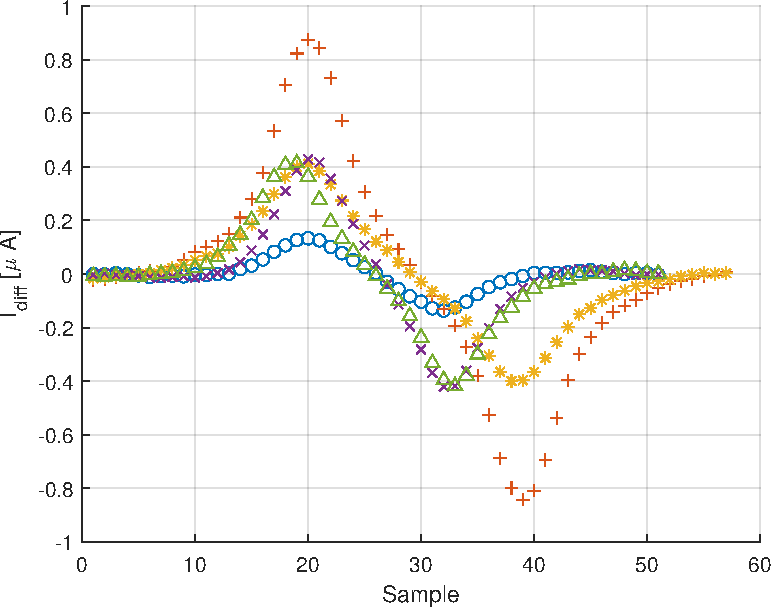
\includegraphics[width=.95\linewidth]{signal_visualization_fig.pdf}
	\caption{}
\end{subfigure}
\caption{}
\label{fig:generale}
\end{figure*}

Il citometro ad impedenza è un dispositivo COMPLETA COMPLETA

Ovvero n on è altro che un microcanale riempito di un buffer conduttivo al cui interno passano delle correnti elettriche. Nel dispositivo in questione si applica un potenziale all'elettrodo centrale e si misura una corrente differenziale tra i due elettrodi laterali.

METTI CREF FIGURA

Tramite la misura di corrente differenziale è possibile stimare alcune proprietà della cellula che passa nel canale. In particolare, al passaggio delle cellula, si misura un segnale con una forma d'onda di tipo gaussiana bipolare.

Tramite il segnale di picco è possibile stimare il diametro. Il segnale è proporzionale al volume della cellula per cui il diametro sarà legato all'ampiezza del segnale ($a$) come:


\begin{equation}
	D=G a^{1 / 3}
\end{equation}

Dove $G$ è un guadagno che risente delle proprietà elettriche del citometro.

\subsection{Gaussiana bipolare}

\begin{figure}
		\centering
		\footnotesize{ \def\svgwidth{0.95\linewidth}
			\input{bipolarGaussian.pdf_tex}}
	\caption{}
	\label{fig:gaussiana}
\end{figure}


La gaussiana bipolare è una forma d'onda caratteristica composta da due gaussiane identificata dalla generica equazione:

\begin{equation}
	g(t)=a\left[e^{g_{+}(t)}-e^{g_{-}(t)}\right]
	\label{eq:gaussianabipolare}
\end{equation}

Ovvero, considerata un'ampiezza di riferimento $a$ (i.e. il valore massimo di picco), è la somma di due gaussiane nel tempo di cui la seconda ribaltata. La distanza picco-picco è pari a $\delta$ e si introduce un parametro di centratura $t_c$. Le due gaussiane condividono la medesima deviazione standard $\sigma$ e sono identificate dall'equazione:

\begin{equation}
	g_{\pm}(t)=\frac{-\left(t-\left(t_{c} \pm(\delta / 2)\right)\right)^{2}}{2 \sigma^{2}}
\end{equation}

Dove il segno $\pm$ va riferimento alla gaussiana positiva o ribaltata.

\subsection{Procedura di fitting}

Partendo dai dati sperimentali è necessario introdurre una procedura di fitting numerico per identificare la gaussiana, e quindi i suoi quattro parametri descrittivi, tale da rappresentare il segnale analizzato.

Tale procedura di fitting viene implmentata secondo un algoritmo di ottimizzazione. Ovvero, si cerca di ridurre la differenza tra il dato misurato $[d]_i$ e il template di fitting ($g$) allo stesso instante temporale. 

Definita la funzione di errore come tale differenza:

\begin{equation}
	\underline{e}=[d]_{i}-g_{i}\left(t_{i}, a,t_c,\delta,\sigma\right)
\end{equation}

Si cerca di minimizzare la funzione obiettivo definita proprio come la norma dell'errore:

\begin{equation}
	\mathrm{E}(a,t_c,\delta,\sigma) = \frac{1}{2} \sum_{i}\left\|d_{i}-g\left(t_{i},a,t_c,\delta,\sigma\right)\right\|^{2}
\end{equation}


\subsection{Accuratezza}


I dispositivi microfluidi possono essere più o meno accurati. Questo è legato alla configurazione degli elettrodi, alla geometria e COMPLETA COMPLETA

In particolare, per il caso di riferimento si osserva una dipendenza del segnale dalla posizione all'interno del canale. Nonostante l'ampiezza del picco della gaussiana sia correlata con il diametro cellulare si osserva una dipendenza anche dalla posizione.

Ovvero, a parità di diametro, una cellula passante vicino agli elettrodi darà un picco di ampiezza maggiore alla stessa cellula passante ad una distanza maggiore.

Nonostante nella configurazione utilizzata non si può avere una misura diretta della posizione all'interno del canale è possibile ottenerne una stima effettuando una compensazione del segnale tenendo conto della correlazione tra la posizione e lo shape parameters.

In particolare, risulta valida la relazione tra il parametro di forma $\sigma \over \delta$ e il diametro normalizzato che segue una legge lineare:
\begin{equation}
	{D\over d}={c_1+c_2\left(\sigma \over \delta \right)}
	\label{eq:compensazione}
\end{equation}

Si possono quindi usare tali coefficienti della retta per correggere il diametro elettrico togliendo l'effetto di posizione \cite{errico_mitigating_2017}.


%\begin{figure}[t!]
%	\centering
%	\includegraphics[width=0.95\linewidth]{imagefile}
%	\caption{}
%	\label{fig:}
%\end{figure}

\begin{figure}[t!]
	\centering
	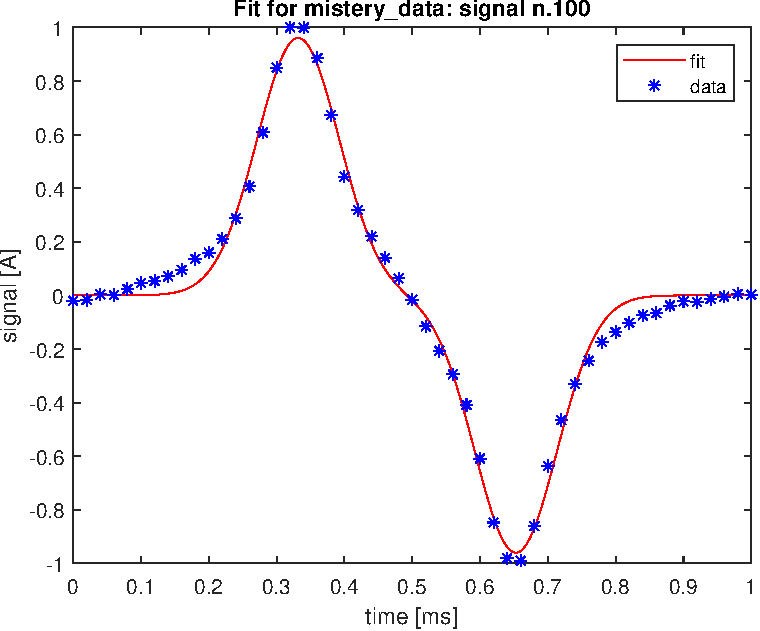
\includegraphics[width=0.9\linewidth]{fitted}
	\caption{Grafico dell'andamento temporale del segnale n. 100. In blu i campioni e in rosso il segnale fittato con una gaussiana bipolare}
	\label{fig:fitted}
\end{figure}


\begin{figure}[t!]
	\centering
	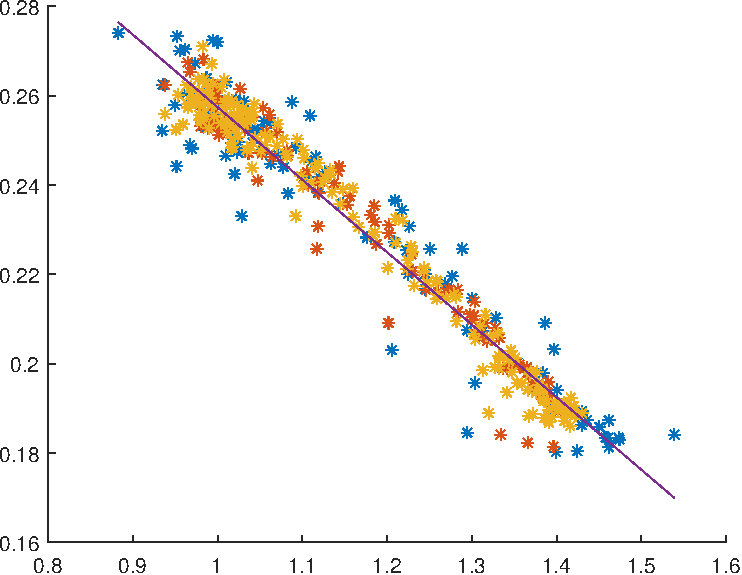
\includegraphics[width=0.9\linewidth]{normalized_diam_figs}
	\caption{}
	\label{fig:normalized}
\end{figure}

\begin{figure*}[t!]
	\centering
	\begin{subfigure}{0.5\linewidth}
			\centering
	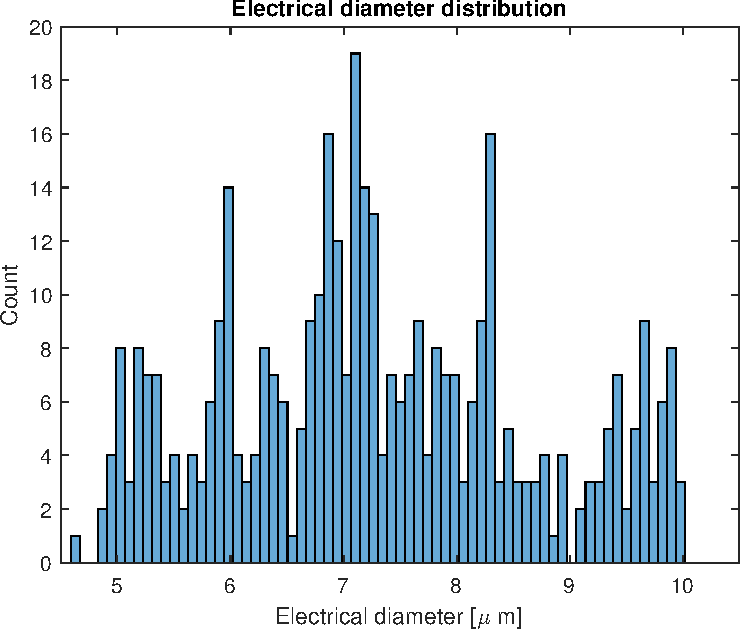
\includegraphics[width=0.9\linewidth]{histogram_figs}
\caption{}
	\end{subfigure}\hfill
\begin{subfigure}{0.5\linewidth}
		\centering
	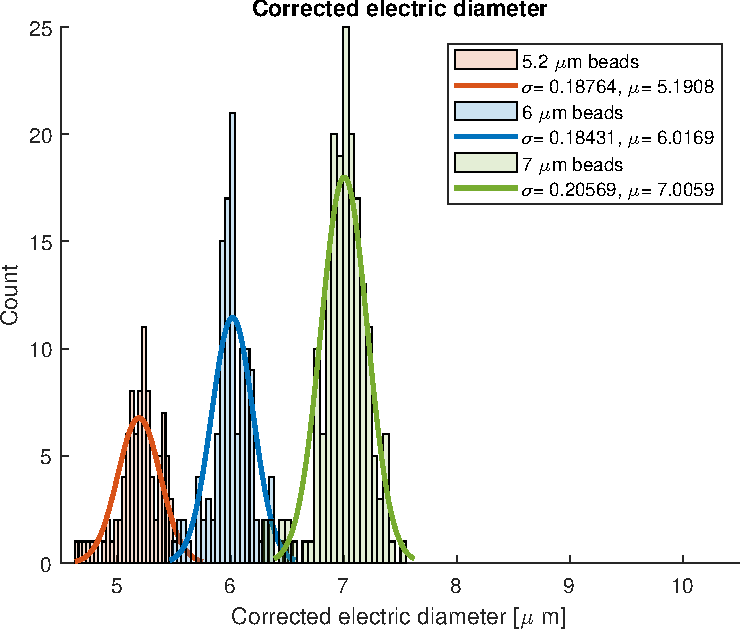
\includegraphics[width=0.9\linewidth]{histogram_corrected2_fig}
	\caption{}
\end{subfigure}
	\caption{}
	\label{fig:histogram}
\end{figure*}

\begin{figure*}[t!]
	\centering
	\begin{subfigure}{0.5\linewidth}
			\centering
		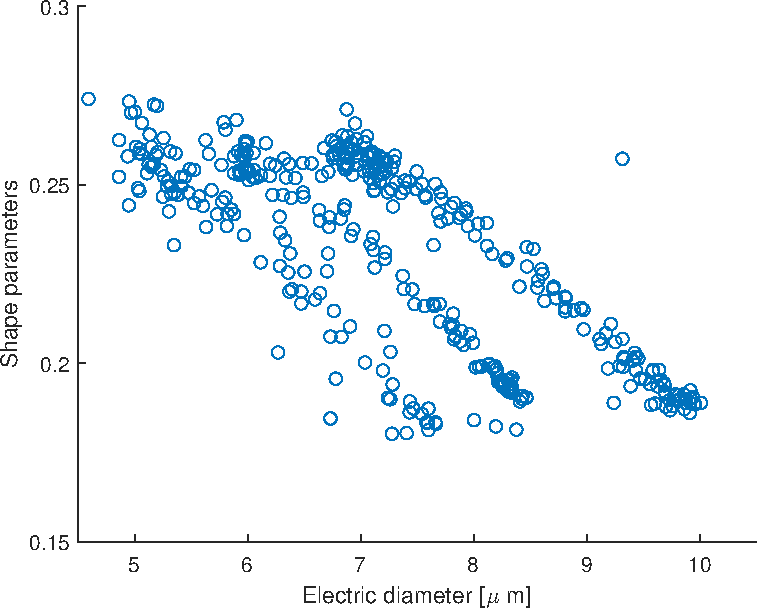
\includegraphics[width=0.9\linewidth]{scatter_fig}
		\caption{}
		\label{fig:scatter_init}
	\end{subfigure}\hfill
	\begin{subfigure}{0.5\linewidth}
			\centering
		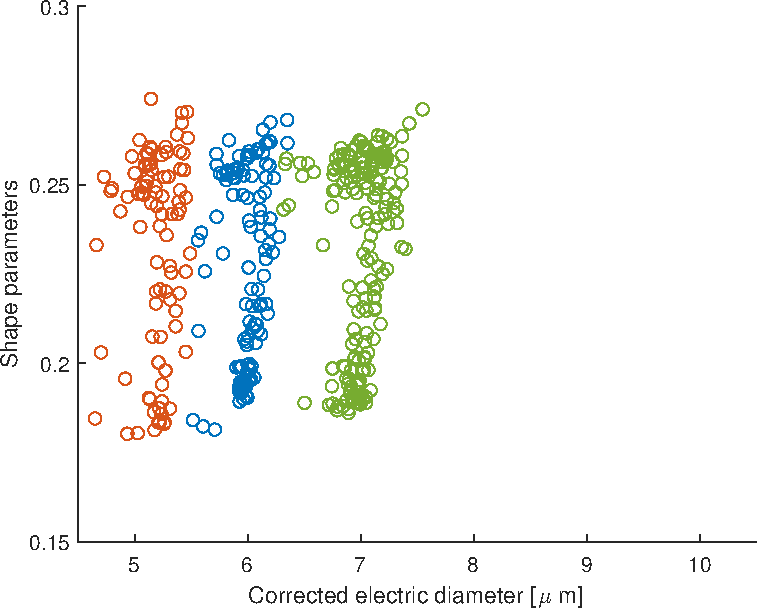
\includegraphics[width=0.9\linewidth]{scatter_corrected2_fig}
		\caption{}
	\end{subfigure}
	\caption{}
	\label{fig:scatter}
\end{figure*}


\begin{figure*}[t!]
	\centering
	\begin{subfigure}{0.5\linewidth}
		\centering
		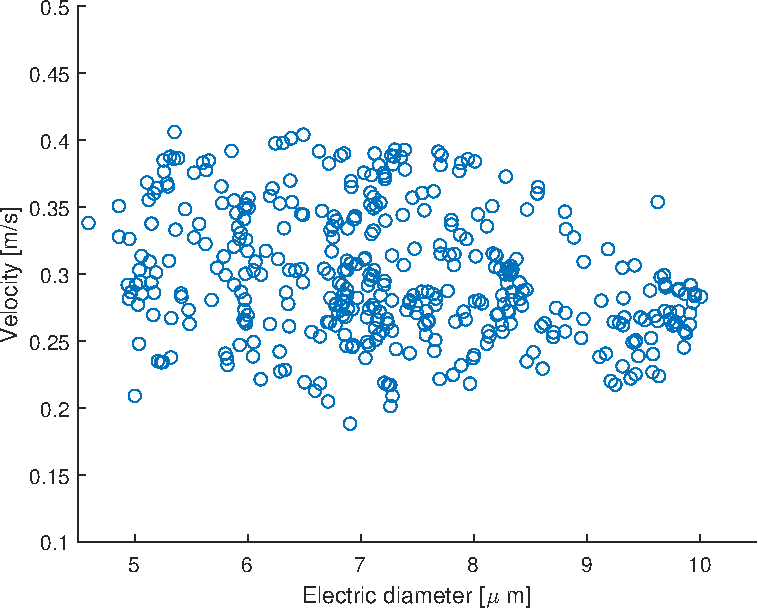
\includegraphics[width=0.9\linewidth]{velocity_fig}
		\caption{}
	\end{subfigure}\hfill
	\begin{subfigure}{0.5\linewidth}
		\centering
		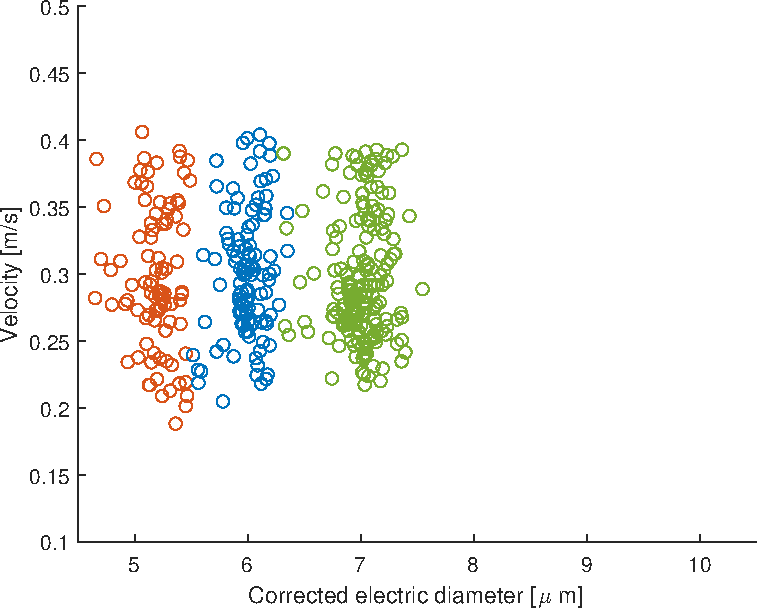
\includegraphics[width=0.9\linewidth]{velocity_corrected_fig}
		\caption{}
	\end{subfigure}
	\caption{}
	\label{fig:velocity}
\end{figure*}




\begin{figure*}[t!]
	\centering
		\begin{subfigure}{0.33\linewidth}
		\centering
		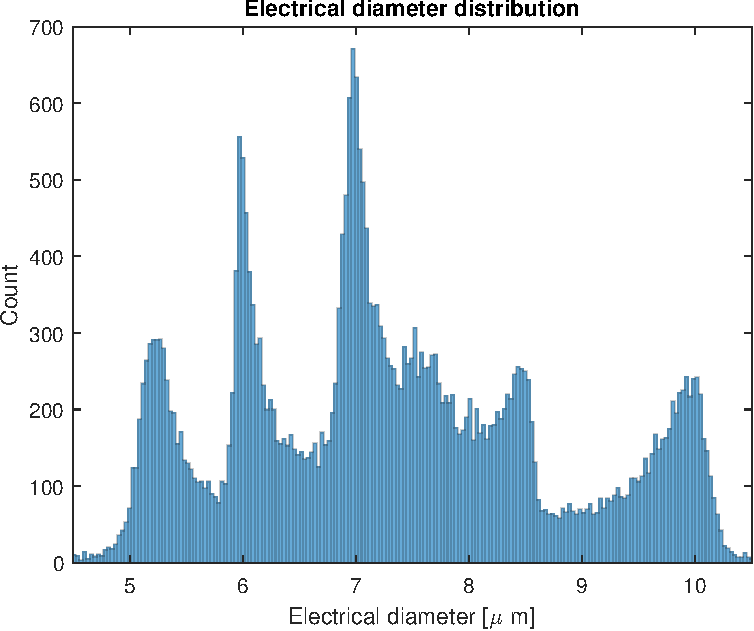
\includegraphics[width=0.9\linewidth]{histogram_data}
		\caption{}
	\end{subfigure}\hfill
	\begin{subfigure}{0.33\linewidth}
		\centering
		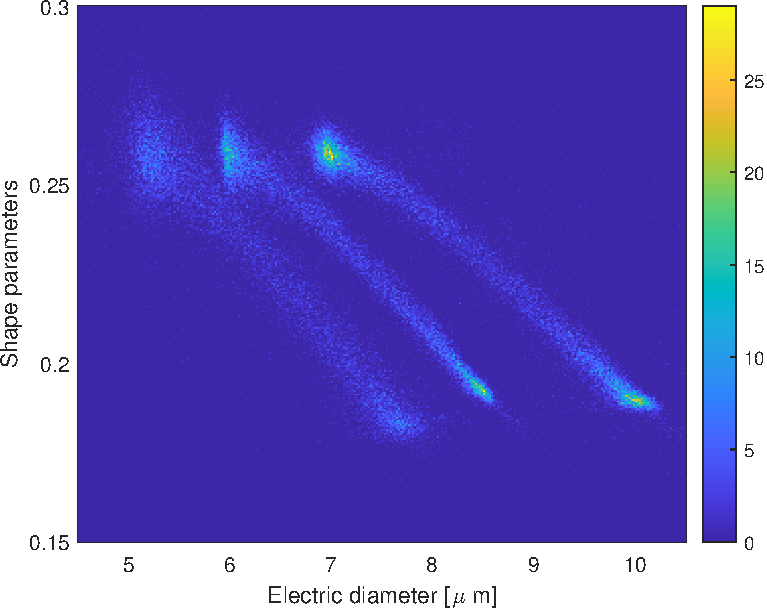
\includegraphics[width=0.9\linewidth]{density_diam_shape}
		\caption{}
	\end{subfigure}\hfill
	\begin{subfigure}{0.33\linewidth}
		\centering
		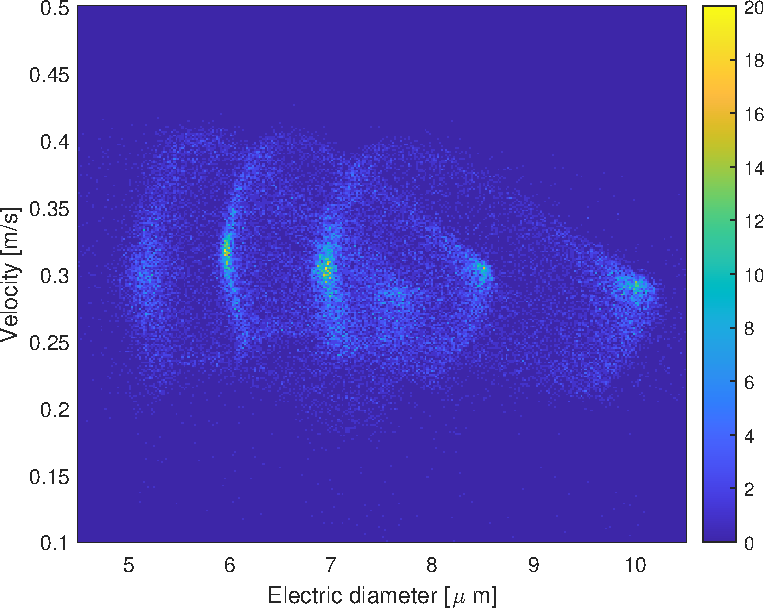
\includegraphics[width=0.9\linewidth]{density_diam_velocity}
		\caption{}
	\end{subfigure}\hfill
	\begin{subfigure}{0.33\linewidth}
	\centering
	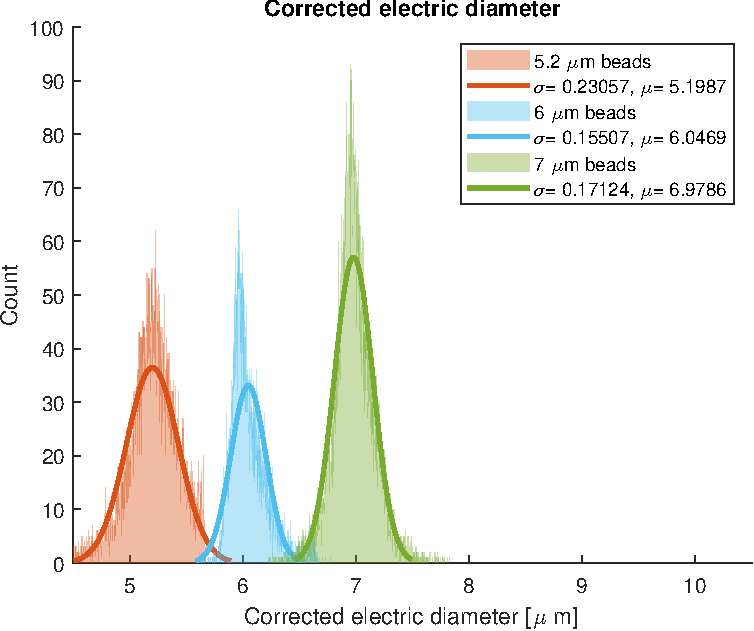
\includegraphics[width=0.9\linewidth]{histogram_corrected_fig}
	\caption{}
\end{subfigure}\hfill
	\begin{subfigure}{0.33\linewidth}
	\centering
	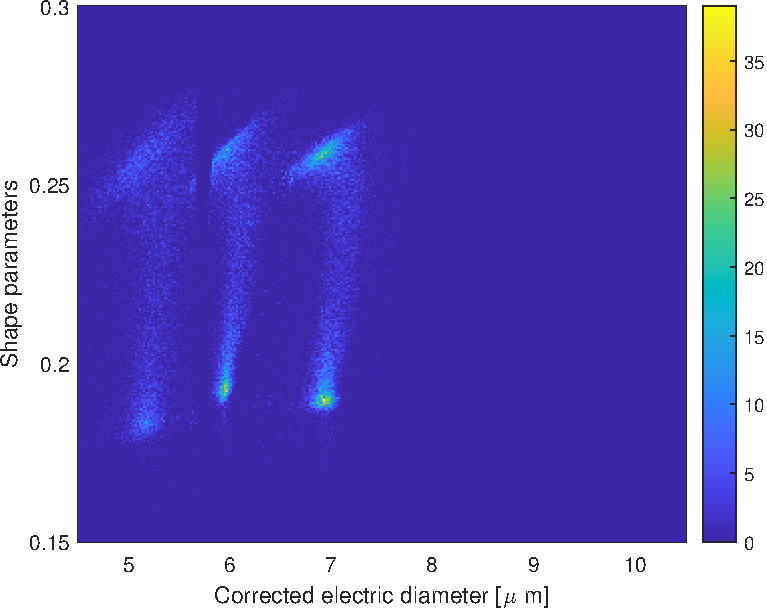
\includegraphics[width=0.9\linewidth]{density_diam_corr_shape}
	\caption{}
\end{subfigure}\hfill
\begin{subfigure}{0.33\linewidth}
	\centering
	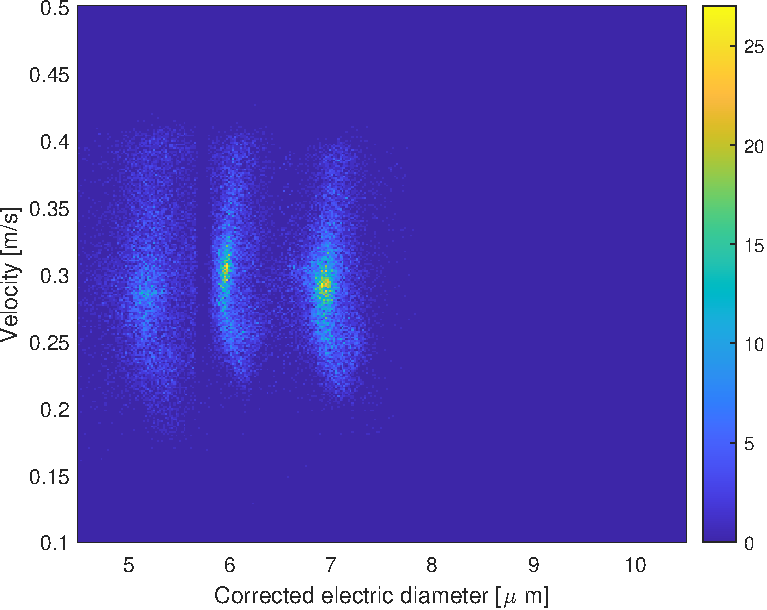
\includegraphics[width=0.9\linewidth]{density_diam_corr_velocity}
	\caption{}
\end{subfigure}
	\caption{}
	\label{fig:density}
\end{figure*}

\begin{figure}[t!]
	\centering
	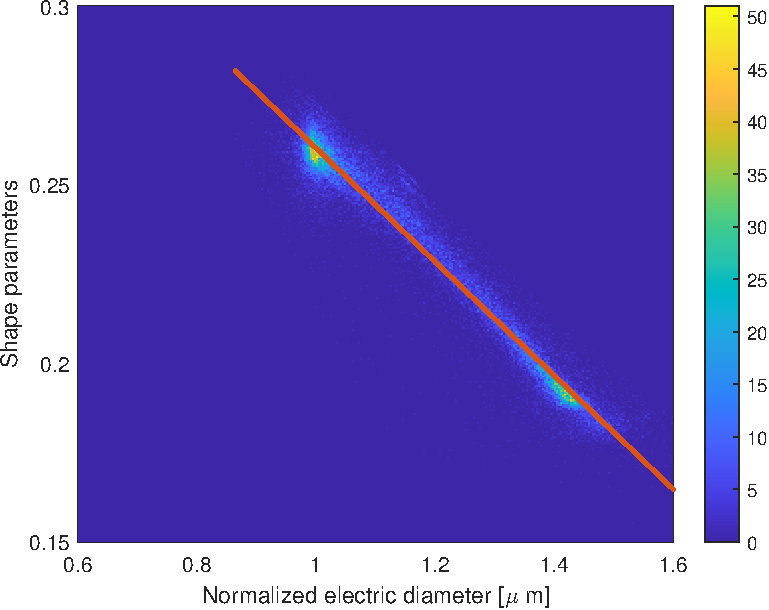
\includegraphics[width=0.9\linewidth]{normalized_D}
	\caption{}
	\label{fig:normalizedDensity}
\end{figure}



\subsection{Dataset di riferimento}

Il dataset di riferimento è un insieme di dati grezzi di citometro ad impedenza.  

Per il dispositivo in questione il guadagno è pari a 10.5 $\mu$m / A\textsuperscript{1/3}. I segnali sono campionati con una frequenza $f_s=115$ kHz con un totale di oltre 50.000 segnali.


PARLA DEL DATASET E DEI PARAMETRI 

\section{Risultati}

Inizialmente la procedura viene applicata su un dataset ristretto considerando 400 segnali. Vengono selezionati quindi i segnali di indice da 400 a 800.

Successivamente la procedura verrà applicata anche su un riferimento più esteso.

\subsection{Fitting numerico}

A partire dal singolo segnale all'interno dell'intero dataset è possibile fittare la gaussiana bipolare andando a stimarne i quattro coefficienti descrittivi.

Considerando il template in \cref{eq:gaussianabipolare} è possibile utilizzare il comando Matlab \texttt{fit()} fornendo il template stesso, i dati e i valori iniziali per la stima ai minimi quadrati.

Inoltre, essendo il segnale molto piccolo $\propto 10^{-6}$ è utile normalizzare il segnale di ampiezza e scalare l'asse dei tempi riportandolo in secondi nel range $[0;\:{1\over f_s}]$, dove $f_s$ è la frequenza di campionamento il cui inverso indica l'ultimo campione temporale.

A questo deve seguire poi necessariamente una riscalatura nel dominio originario. 

Un esempio di fitting è presente in \cref{fig:fitted}.


\subsection{Compensazione}

Per la procedura di compensazione è necessario stimare i coefficienti di un fitting lineare. Tale fitting deve essere fatto nello spazio $[{\delta\over \sigma};\:{D\over d}$] ed è quindi necessario normalizzare i diametri elettrici rispetto i singoli diametri nominali delle tre famiglie. 

Dallo scatter plot del diametro elettrico vs shape parameters è possibile distinguere tre famiglie (\cref{fig:scatter_init}). Mediante la funzione \texttt{inpolygon()} è possibile selezionare separatamente i valori corrispondenti alle tre famiglie e quindi normalizzarle per il rispettivo diametro nominale. 

Quindi è possibile calcolare la retta che meglio approssima l'andamento dello shape parameter in funzione del diametro elettrico normalizzato (\cref{fig:normalized}). Dunque è possibile estrarre i coefficienti:
\begin{itemize}
	\item $\mathtt{c1}=2.59$
	\item $\mathtt{c2}=-6.20$
\end{itemize}

E il coefficiente di determinazione $\mathtt{r}^2=0.96$. 

Tramite tali coefficienti è possibile correggere i valori tramite l'\cref{eq:compensazione}.

Si ottengono quindi le famiglie separate sia nello scatter plot dello shape parameter che della velocità, in \cref{fig:scatter} e \cref{fig:velocity}.


\subsection{Estensione del dominio di interesse}

La stessa procedura può essere applicata anche su una quantità di segnali notevolmente maggiore. Vengono quindi considerati, nello stesso dataset di riferimento, i segnali di indice a 200 a 35200. 

La procedura può essere applicata allo stesso modo ma gli scatter plot vengono sostituiti da plot di densità che permettono di osservare meglio la distribuzione dei valori.


\section{Conclusioni}


%\pagebreak
\section*{Disponibilità dei dati}

Il materiale è disponibile alla repository online del progetto: \url{https://github.com/mastroalex/curve-fitting}


\raggedbottom
%\pagebreak
\printbibliography[title=Riferimenti]
%\section*{References}


\clearpage
\onecolumn
\section*{Appendice}






\end{document}